\section{Kết quả}

\subsection{Kết quả huấn luyện mô hình CNN}

\subsubsection{Kết quả kiểm định chéo 5 phần}

\begin{table}[H]
\centering
\caption{Kết quả kiểm định chéo 5 phần (5-Fold Cross Validation)}
\label{tab:cv_results}
\begin{tabular}{|c|c|c|}
\hline
\textbf{Fold} & \textbf{Accuracy} & \textbf{F1-Score} \\
\hline
Fold 1 & 98.34\% & 98.34\% \\
\hline
Fold 2 & 98.57\% & 98.57\% \\
\hline
Fold 3 & 98.10\% & 98.10\% \\
\hline
Fold 4 & 97.86\% & 97.86\% \\
\hline
Fold 5 & 97.86\% & 97.86\% \\
\hline
\textbf{Mean ± Std} & \textbf{98.15\% ± 0.28\%} & \textbf{98.15\% ± 0.28\%} \\
\hline
\end{tabular}
\end{table}

Kết quả Cross Validation cho thấy sự ổn định của mô hình: độ lệch chuẩn của Accuracy chỉ khoảng 0.28\%, Accuracy từng fold đều vượt ngưỡng 97.8\%, và điều này cho thấy không có dấu hiệu Overfitting nghiêm trọng, tức Accuracy trên tập validation phản ánh tốt khả năng tổng quát hóa của mô hình.

\begin{figure}[H]
    \centering
    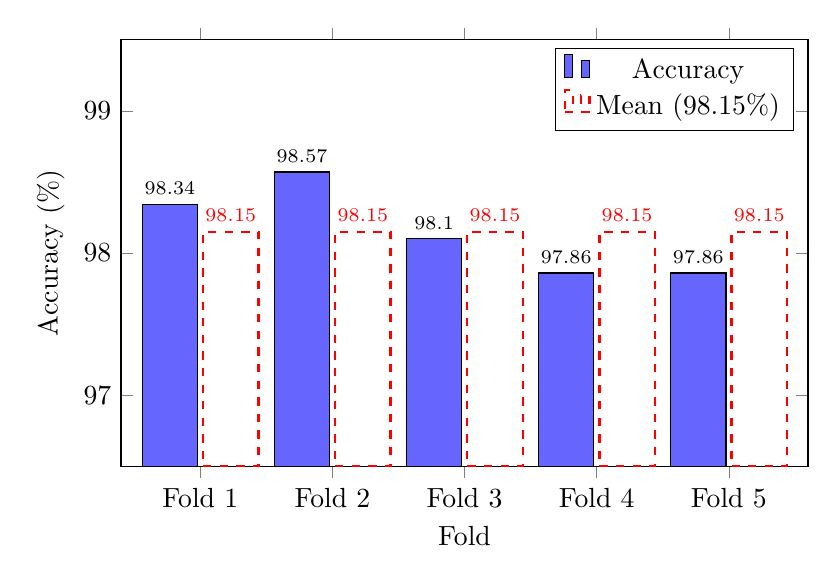
\begin{tikzpicture}
        \begin{axis}[
            ybar,
            width=0.85\textwidth,
            height=7cm,
            ylabel={Accuracy (\%)},
            xlabel={Fold},
            symbolic x coords={Fold 1, Fold 2, Fold 3, Fold 4, Fold 5},
            xtick=data,
            ymin=96.5,
            ymax=99.5,
            bar width=20pt,
            nodes near coords,
            nodes near coords align={vertical},
            every node near coord/.append style={font=\scriptsize},
            enlarge x limits=0.15,
        ]
        \addplot[fill=blue!60] coordinates {
            (Fold 1, 98.34)
            (Fold 2, 98.57)
            (Fold 3, 98.10)
            (Fold 4, 97.86)
            (Fold 5, 97.86)
        };
        % Đường trung bình
        \addplot[red, thick, dashed, domain=0:5] coordinates {
            (Fold 1, 98.15) (Fold 2, 98.15) (Fold 3, 98.15) (Fold 4, 98.15) (Fold 5, 98.15)
        };
        \legend{Accuracy, Mean (98.15\%)}
        \end{axis}
    \end{tikzpicture}
    \caption{So sánh Accuracy giữa các fold trong Cross Validation}
    \label{fig:cv_comparison}
\end{figure}

\subsubsection{Kết quả trên tập kiểm tra}

\begin{table}[H]
\centering
\caption{Các chỉ số đánh giá trên tập kiểm tra (526 mảnh)}
\label{tab:test_metrics}
\begin{tabular}{|l|c|c|}
\hline
\textbf{Metric} & \textbf{Value} & \textbf{Percent} \\
\hline
\textbf{Accuracy} & 0.9886 & \textbf{98.86\%} \\
\hline
Precision (macro avg) & 0.9886 & 98.86\% \\
\hline
Recall (macro avg) & 0.9886 & 98.86\% \\
\hline
F1-Score (macro avg) & 0.9886 & 98.86\% \\
\hline
ROC-AUC (macro avg) & 0.9998 & 99.98\% \\
\hline
\end{tabular}
\end{table}

\begin{figure}[H]
    \centering
    \begin{tikzpicture}
        % Định nghĩa màu sắc Blues colormap (từ nhạt đến đậm)
        \definecolor{blue0}{RGB}{247,251,255}
        \definecolor{blue1}{RGB}{222,235,247}
        \definecolor{blue2}{RGB}{198,219,239}
        \definecolor{blue3}{RGB}{158,202,225}
        \definecolor{blue4}{RGB}{107,174,214}
        \definecolor{blue5}{RGB}{66,146,198}
        \definecolor{blue6}{RGB}{33,113,181}
        \definecolor{blue7}{RGB}{8,81,156}
        \definecolor{blue8}{RGB}{8,48,107}

        % Kích thước ô
        \def\cellsize{1.8}

        % Vẽ các ô với màu Blues gradient
        % Hàng 0 (Rừng ổn định): 129, 2, 0, 0
        \fill[blue8] (0*\cellsize, 3*\cellsize) rectangle (1*\cellsize, 4*\cellsize);
        \fill[blue1] (1*\cellsize, 3*\cellsize) rectangle (2*\cellsize, 4*\cellsize);
        \fill[blue0] (2*\cellsize, 3*\cellsize) rectangle (3*\cellsize, 4*\cellsize);
        \fill[blue0] (3*\cellsize, 3*\cellsize) rectangle (4*\cellsize, 4*\cellsize);

        % Hàng 1 (Mất rừng): 4, 126, 0, 0
        \fill[blue1] (0*\cellsize, 2*\cellsize) rectangle (1*\cellsize, 3*\cellsize);
        \fill[blue8] (1*\cellsize, 2*\cellsize) rectangle (2*\cellsize, 3*\cellsize);
        \fill[blue0] (2*\cellsize, 2*\cellsize) rectangle (3*\cellsize, 3*\cellsize);
        \fill[blue0] (3*\cellsize, 2*\cellsize) rectangle (4*\cellsize, 3*\cellsize);

        % Hàng 2 (Phi rừng): 0, 0, 133, 0
        \fill[blue0] (0*\cellsize, 1*\cellsize) rectangle (1*\cellsize, 2*\cellsize);
        \fill[blue0] (1*\cellsize, 1*\cellsize) rectangle (2*\cellsize, 2*\cellsize);
        \fill[blue8] (2*\cellsize, 1*\cellsize) rectangle (3*\cellsize, 2*\cellsize);
        \fill[blue0] (3*\cellsize, 1*\cellsize) rectangle (4*\cellsize, 2*\cellsize);

        % Hàng 3 (Phục hồi rừng): 0, 0, 0, 132
        \fill[blue0] (0*\cellsize, 0*\cellsize) rectangle (1*\cellsize, 1*\cellsize);
        \fill[blue0] (1*\cellsize, 0*\cellsize) rectangle (2*\cellsize, 1*\cellsize);
        \fill[blue0] (2*\cellsize, 0*\cellsize) rectangle (3*\cellsize, 1*\cellsize);
        \fill[blue8] (3*\cellsize, 0*\cellsize) rectangle (4*\cellsize, 1*\cellsize);

        % Vẽ đường viền cho các ô
        \draw[white, line width=1pt] (0,0) grid[step=\cellsize] (4*\cellsize, 4*\cellsize);

        % Thêm số liệu vào các ô
        \node[font=\normalsize\bfseries, text=white] at (0.5*\cellsize, 3.5*\cellsize) {129};
        \node[font=\normalsize, text=black] at (1.5*\cellsize, 3.5*\cellsize) {2};
        \node[font=\normalsize, text=black] at (2.5*\cellsize, 3.5*\cellsize) {0};
        \node[font=\normalsize, text=black] at (3.5*\cellsize, 3.5*\cellsize) {0};

        \node[font=\normalsize, text=black] at (0.5*\cellsize, 2.5*\cellsize) {4};
        \node[font=\normalsize\bfseries, text=white] at (1.5*\cellsize, 2.5*\cellsize) {126};
        \node[font=\normalsize, text=black] at (2.5*\cellsize, 2.5*\cellsize) {0};
        \node[font=\normalsize, text=black] at (3.5*\cellsize, 2.5*\cellsize) {0};

        \node[font=\normalsize, text=black] at (0.5*\cellsize, 1.5*\cellsize) {0};
        \node[font=\normalsize, text=black] at (1.5*\cellsize, 1.5*\cellsize) {0};
        \node[font=\normalsize\bfseries, text=white] at (2.5*\cellsize, 1.5*\cellsize) {133};
        \node[font=\normalsize, text=black] at (3.5*\cellsize, 1.5*\cellsize) {0};

        \node[font=\normalsize, text=black] at (0.5*\cellsize, 0.5*\cellsize) {0};
        \node[font=\normalsize, text=black] at (1.5*\cellsize, 0.5*\cellsize) {0};
        \node[font=\normalsize, text=black] at (2.5*\cellsize, 0.5*\cellsize) {0};
        \node[font=\normalsize\bfseries, text=white] at (3.5*\cellsize, 0.5*\cellsize) {132};

        % Nhãn cột (Dự đoán) - xoay nghiêng
        \node[font=\scriptsize, rotate=45, anchor=east] at (0.5*\cellsize, -0.2*\cellsize) {Rừng ổn định};
        \node[font=\scriptsize, rotate=45, anchor=east] at (1.5*\cellsize, -0.2*\cellsize) {Mất rừng};
        \node[font=\scriptsize, rotate=45, anchor=east] at (2.5*\cellsize, -0.2*\cellsize) {Phi rừng};
        \node[font=\scriptsize, rotate=45, anchor=east] at (3.5*\cellsize, -0.2*\cellsize) {Phục hồi rừng};
        \node[font=\small\bfseries] at (2*\cellsize, -1.1*\cellsize) {Dự đoán};

        % Nhãn hàng (Thực tế)
        \node[font=\scriptsize, anchor=east] at (-0.1*\cellsize, 3.5*\cellsize) {Rừng ổn định};
        \node[font=\scriptsize, anchor=east] at (-0.1*\cellsize, 2.5*\cellsize) {Mất rừng};
        \node[font=\scriptsize, anchor=east] at (-0.1*\cellsize, 1.5*\cellsize) {Phi rừng};
        \node[font=\scriptsize, anchor=east] at (-0.1*\cellsize, 0.5*\cellsize) {Phục hồi rừng};
        \node[font=\small\bfseries, rotate=90] at (-1.5*\cellsize, 2*\cellsize) {Thực tế};

        % Thanh màu (color bar) - Blues gradient (9 segments, mỗi segment = 4/9 cellsize)
        \pgfmathsetmacro{\segheight}{4/9}
        \foreach \i/\col in {0/blue0, 1/blue1, 2/blue2, 3/blue3, 4/blue4, 5/blue5, 6/blue6, 7/blue7, 8/blue8} {
            \fill[\col] (5*\cellsize, \i*\segheight*\cellsize) rectangle (5.4*\cellsize, \i*\segheight*\cellsize+\segheight*\cellsize);
        }
        \draw[black, thin] (5*\cellsize, 0) rectangle (5.4*\cellsize, 4*\cellsize);
        \node[font=\tiny, anchor=west] at (5.5*\cellsize, 0) {0};
        \node[font=\tiny, anchor=west] at (5.5*\cellsize, 1*\cellsize) {40};
        \node[font=\tiny, anchor=west] at (5.5*\cellsize, 2*\cellsize) {80};
        \node[font=\tiny, anchor=west] at (5.5*\cellsize, 3*\cellsize) {120};
    \end{tikzpicture}
    \caption{Confusion Matrix dạng heatmap trên tập kiểm tra (n=526, Accuracy: 98.86\%)}
    \label{fig:confusion_heatmap}
\end{figure}

\begin{table}[H]
\centering
\caption{Phân tích chi tiết từng lớp}
\label{tab:class_analysis}
\begin{tabular}{|l|c|c|c|c|c|}
\hline
\textbf{Lớp} & \textbf{Precision} & \textbf{Recall} & \textbf{F1-Score} & \textbf{Samples} & \textbf{Errors} \\
\hline
0 - Rừng ổn định & 96.99\% & 98.47\% & 97.73\% & 131 & 4 FP, 2 FN \\
\hline
1 - Mất rừng & 98.44\% & 96.92\% & 97.67\% & 130 & 2 FP, 4 FN \\
\hline
2 - Phi rừng & 100.00\% & 100.00\% & 100.00\% & 133 & 0 \\
\hline
3 - Phục hồi rừng & 100.00\% & 100.00\% & 100.00\% & 132 & 0 \\
\hline
\end{tabular}
\end{table}

\textit{Ghi chú: FP = False Positive (dương tính giả), FN = False Negative (âm tính giả)}

Tổng cộng chỉ có 6/526 mẫu bị phân loại sai, tương đương tỷ lệ lỗi 1.14\%. Trong đó, hai mẫu thuộc Lớp 0 (Rừng ổn định) bị nhầm thành Lớp 1 (Mất rừng) và bốn mẫu thuộc Lớp 1 (Mất rừng) bị nhầm thành Lớp 0 (Rừng ổn định). Đánh giá chi tiết cho thấy Lớp 2 (Phi rừng) và Lớp 3 (Phục hồi rừng) được phân loại hoàn hảo với Accuracy 100\%.

Việc nhầm lẫn chỉ xảy ra giữa hai lớp Rừng ổn định (Lớp 0) và Mất rừng (Lớp 1) có thể được giải thích bởi các yếu tố sau. Thứ nhất, về \textbf{sự tương đồng về đặc trưng quang phổ}, cả hai lớp đều có sự hiện diện của rừng ở ít nhất một thời điểm; các khu vực rừng bị suy thoái nhẹ có thể có phổ phản xạ đặc trưng tương tự với rừng ổn định, đặc biệt khi mức độ mất rừng không rõ ràng. Thứ hai, về \textbf{hiệu ứng biên}, tại ranh giới giữa vùng rừng và vùng mất rừng, các điểm ảnh có thể chứa cả hai loại lớp phủ (điểm ảnh hỗn hợp), dẫn đến vector đặc trưng không điển hình cho một lớp cụ thể. Thứ ba, về \textbf{biến động theo mùa}, một số khu vực rừng ngập mặn có thể có biến động theo mùa về mật độ tán lá, tạo ra sự thay đổi NDVI tương tự như mất rừng nhưng thực tế là biến động tự nhiên. Thứ tư, về \textbf{độ phân giải thời gian}, với chỉ hai thời điểm quan sát, một số biến động ngắn hạn hoặc phục hồi nhanh có thể không được ghi nhận chính xác.

Tuy nhiên, với tỷ lệ nhầm lẫn rất thấp (chỉ 6/526 mẫu, ~1.14\%), mô hình vẫn đạt hiệu quả cao trong việc phân biệt các lớp biến động rừng.

\subsubsection{Đường cong ROC}

\begin{table}[H]
\centering
\caption{Điểm ROC-AUC cho từng lớp trên tập kiểm tra}
\label{tab:roc_auc}
\begin{tabular}{|l|c|}
\hline
\textbf{Lớp} & \textbf{ROC-AUC} \\
\hline
0 - Rừng ổn định & 0.9998 \\
\hline
1 - Mất rừng & 0.9997 \\
\hline
2 - Phi rừng & 1.0000 \\
\hline
3 - Phục hồi rừng & 1.0000 \\
\hline
\textbf{Trung bình macro} & \textbf{0.9998} \\
\hline
\end{tabular}
\end{table}

\begin{figure}[H]
    \centering
    \begin{tikzpicture}
        \begin{axis}[
            width=0.75\textwidth,
            height=8cm,
            xlabel={False Positive Rate (FPR)},
            ylabel={True Positive Rate (TPR)},
            xmin=0, xmax=1,
            ymin=0, ymax=1,
            legend pos=south east,
            legend style={font=\small},
            grid=major,
            grid style={dashed, gray!30},
        ]
        % Đường chéo (phân loại ngẫu nhiên)
        \addplot[gray, dashed, thick] coordinates {(0,0) (1,1)};

        % Đường cong ROC cho 4 lớp (mô phỏng dựa trên AUC cao)
        % Lớp 0 - Rừng ổn định (AUC = 0,9998)
        \addplot[green!60!black, thick] coordinates {
            (0,0) (0,0.95) (0.001,0.98) (0.002,0.99) (0.01,0.995) (0.05,0.998) (1,1)
        };
        % Lớp 1 - Mất rừng (AUC = 0,9997)
        \addplot[red!70, thick] coordinates {
            (0,0) (0,0.94) (0.001,0.97) (0.003,0.99) (0.01,0.994) (0.05,0.997) (1,1)
        };
        % Lớp 2 - Phi rừng (AUC = 1,0000)
        \addplot[blue!60, thick] coordinates {
            (0,0) (0,1) (1,1)
        };
        % Lớp 3 - Phục hồi rừng (AUC = 1,0000)
        \addplot[orange!80, thick] coordinates {
            (0,0) (0,1) (1,1)
        };

        \legend{Ngẫu nhiên, Rừng ổn định, Mất rừng, Phi rừng, Phục hồi rừng}
        \end{axis}
    \end{tikzpicture}
    \caption{Đường cong ROC cho các lớp phân loại}
    \label{fig:roc_curves}
\end{figure}

\subsection{Kết quả phân loại toàn bộ vùng nghiên cứu}

\subsubsection{Thống kê phân loại}

\begin{table}[H]
\centering
\caption{Phân bố diện tích theo lớp phân loại}
\label{tab:area_distribution}
\begin{tabular}{|c|l|r|r|r|r|}
\hline
\textbf{Lớp} & \textbf{Tên lớp} & \textbf{Số pixels} & \textbf{Tỷ lệ (\%)} & \textbf{Diện tích (ha)} & \textbf{Diện tích (km²)} \\
\hline
0 & Rừng ổn định & 12,071,691 & 74.30\% & 120,716.91 & 1,207.17 \\
\hline
1 & Mất rừng & 728,215 & 4.48\% & 7,282.15 & 72.82 \\
\hline
2 & Phi rừng & 2,952,854 & 18.17\% & 29,528.54 & 295.29 \\
\hline
3 & Phục hồi rừng & 494,090 & 3.04\% & 4,940.90 & 49.41 \\
\hline
\textbf{Tổng} & & \textbf{16,246,850} & \textbf{100\%} & \textbf{162,468.50} & \textbf{1,624.69} \\
\hline
\end{tabular}
\end{table}

Kết quả từ Bảng~\ref{tab:area_distribution} cho thấy bức tranh tổng quan về tình trạng rừng tại tỉnh Cà Mau trong giai đoạn nghiên cứu. Lớp rừng ổn định chiếm tỷ lệ lớn nhất với 74.30\% (tương đương 1,207.17 km²), phản ánh nỗ lực bảo tồn và quản lý rừng ngập mặn của địa phương, chủ yếu tập trung tại Vườn Quốc gia Mũi Cà Mau và các vùng đệm được bảo vệ nghiêm ngặt. Diện tích mất rừng chiếm 4.48\% (72.82 km²), đây là tỷ lệ đáng quan ngại khi quy đổi ra diện tích tuyệt đối, với các nguyên nhân chính có thể bao gồm chuyển đổi mục đích sử dụng đất sang nuôi trồng thủy sản, xói lở bờ biển do biến đổi khí hậu và tác động của xâm nhập mặn làm suy thoái rừng.

Lớp phi rừng chiếm 18.17\% (295.29 km²), bao gồm các khu vực ao nuôi tôm, đất trống, khu dân cư và cơ sở hạ tầng, phản ánh áp lực phát triển kinh tế - xã hội lên tài nguyên rừng trong khu vực. Lớp phục hồi rừng chiếm 3.04\% (49.41 km²), cho thấy một phần diện tích đã được tái sinh tự nhiên hoặc trồng rừng mới. Mặc dù tỷ lệ phục hồi còn thấp hơn so với diện tích mất rừng, đây vẫn là tín hiệu tích cực cho công tác phục hồi hệ sinh thái rừng ngập mặn trong khu vực.

\begin{figure}[H]
    \centering
    \includegraphics[width=0.95\textwidth]{img/chapter4/Classification.png}
    \caption{Bản đồ phân loại biến động rừng tỉnh Cà Mau}
    \label{fig:classification_map}
\end{figure}

Bản đồ phân loại biến động rừng (Hình~\ref{fig:classification_map}) cho thấy sự phân bố không gian rõ ràng của các lớp phủ. Vùng rừng ổn định (màu xanh lá đậm) tập trung chủ yếu ở phía Tây và Tây Nam của tỉnh, bao gồm khu vực Vườn Quốc gia Mũi Cà Mau và dải rừng phòng hộ ven biển, trong đó sự liên tục của vùng rừng này cho thấy hiệu quả của các chính sách bảo tồn trong khu vực. Vùng mất rừng (màu đỏ) xuất hiện rải rác, chủ yếu tại các khu vực ranh giới giữa rừng và vùng nuôi trồng thủy sản, đặc biệt ở phía Bắc và Đông Bắc của vùng nghiên cứu, phù hợp với thực tế chuyển đổi đất rừng sang ao nuôi tôm trong khu vực.

Vùng phi rừng (màu vàng nhạt) phân bố chủ yếu ở phía Đông và các khu vực nội địa, tương ứng với vùng đầm nuôi thủy sản và đất canh tác nông nghiệp đã tồn tại từ trước giai đoạn nghiên cứu. Vùng phục hồi rừng (màu xanh dương) xuất hiện tại các khu vực ven rừng ổn định, cho thấy quá trình tái sinh tự nhiên hoặc hoạt động trồng rừng đang diễn ra, đặc biệt ở các vùng đệm của khu bảo tồn.

\begin{figure}[H]
    \centering
    \definecolor{stableforest}{HTML}{00734C}
    \definecolor{deforestation}{HTML}{E60000}
    \definecolor{nonforest}{HTML}{FFD37F}
    \definecolor{reforestation}{HTML}{00C5FF}
    \begin{tikzpicture}
        \pie[
            radius=3,
            text=legend,
            color={stableforest, deforestation, nonforest, reforestation},
            explode={0, 0.1, 0, 0}
        ]{
            74.30/Rừng ổn định (74.30\%),
            4.48/Mất rừng (4.48\%),
            18.17/Phi rừng (18.17\%),
            3.04/Phục hồi rừng (3.04\%)
        }
    \end{tikzpicture}
    \caption{Tỷ lệ diện tích các lớp phân loại}
    \label{fig:pie_chart}
\end{figure}

\begin{figure}[H]
    \centering
    \definecolor{stableforest}{HTML}{00734C}
    \definecolor{deforestation}{HTML}{E60000}
    \definecolor{nonforest}{HTML}{FFD37F}
    \definecolor{reforestation}{HTML}{00C5FF}
    \begin{tikzpicture}
        \begin{axis}[
            ybar,
            width=0.85\textwidth,
            height=8cm,
            ylabel={Diện tích (ha)},
            symbolic x coords={Rừng ổn định, Mất rừng, Phi rừng, Phục hồi rừng},
            xtick=data,
            xticklabel style={rotate=15, anchor=east, font=\small},
            nodes near coords,
            nodes near coords align={vertical},
            every node near coord/.append style={font=\scriptsize},
            ymin=0,
            ymax=140000,
            bar width=25pt,
            enlarge x limits=0.2,
        ]
        \addplot[fill=stableforest] coordinates {(Rừng ổn định, 120717)};
        \addplot[fill=deforestation] coordinates {(Mất rừng, 7282)};
        \addplot[fill=nonforest] coordinates {(Phi rừng, 29529)};
        \addplot[fill=reforestation] coordinates {(Phục hồi rừng, 4941)};
        \end{axis}
    \end{tikzpicture}
    \caption{Biểu đồ cột phân bố diện tích theo lớp phân loại}
    \label{fig:area_bar_chart}
\end{figure}

Qua biểu đồ tròn (Hình~\ref{fig:pie_chart}) và biểu đồ cột (Hình~\ref{fig:area_bar_chart}), có thể nhận thấy sự chênh lệch rõ rệt về diện tích giữa các lớp. Rừng ổn định chiếm ưu thế tuyệt đối với hơn 3/4 diện tích vùng nghiên cứu, đây là nền tảng quan trọng cho công tác bảo tồn đa dạng sinh học và phòng hộ ven biển. Đáng chú ý, tỷ lệ mất rừng (4.48\%) vượt quá tỷ lệ phục hồi rừng (3.04\%), cho thấy xu hướng suy giảm ròng của diện tích rừng trong giai đoạn nghiên cứu, với chênh lệch khoảng 1.44\% (tương đương 2,341 ha) là mức độ mất rừng ròng mà khu vực đang phải đối mặt. Diện tích phi rừng lớn (18.17\%) phản ánh mức độ khai thác tài nguyên đất đai trong khu vực, chủ yếu cho hoạt động nuôi trồng thủy sản - ngành kinh tế mũi nhọn của tỉnh Cà Mau.

Cần lưu ý rằng theo khuyến nghị của Olofsson và cộng sự \citeen{olofsson2014}, diện tích ước tính từ bản đồ phân loại cần được hiệu chỉnh dựa trên Confusion Matrix để đảm bảo tính không chệch. Với Accuracy cao của mô hình (98.86\%, Precision và Recall đều trên 96\% cho tất cả các lớp), sai số giữa diện tích thô và diện tích hiệu chỉnh được kỳ vọng là nhỏ. Tuy nhiên, việc thực hiện hiệu chỉnh đầy đủ theo phương pháp Olofsson sẽ là hướng phát triển trong tương lai.

\subsection{So sánh với các nghiên cứu khác}

\subsubsection{So sánh với các công trình trong tài liệu}

\begin{table}[H]
\centering
\caption{So sánh với các nghiên cứu trong tài liệu}
\label{tab:comparison}
\begin{tabular}{|l|l|l|c|c|}
\hline
\textbf{Nghiên cứu} & \textbf{Phương pháp} & \textbf{Dữ liệu} & \textbf{Accuracy} & \textbf{ROC-AUC} \\
\hline
Hansen và cs. (2013) & Decision Trees & Landsat & ~85\% & - \\
\hline
Hethcoat và cs. (2019) & CNN (ResNet) & S1/S2 & 94.3\% & - \\
\hline
Zhang và cs. (2020) & U-Net & Sentinel-2 & 96.8\% & 98.5\% \\
\hline
\textbf{Nghiên cứu này} & \textbf{CNN (custom)} & \textbf{S1/S2} & \textbf{98.86\%} & \textbf{99.98\%} \\
\hline
\end{tabular}
\end{table}

\begin{figure}[H]
    \centering
    \begin{tikzpicture}
        \begin{axis}[
            ybar,
            width=0.9\textwidth,
            height=7cm,
            ylabel={Accuracy (\%)},
            symbolic x coords={Hansen (2013), Hethcoat (2019), Zhang (2020), Nghiên cứu này},
            xtick=data,
            xticklabel style={rotate=15, anchor=east, font=\small},
            ymin=80,
            ymax=102,
            bar width=25pt,
            nodes near coords,
            nodes near coords align={vertical},
            every node near coord/.append style={font=\scriptsize},
            enlarge x limits=0.15,
        ]
        \addplot[fill=teal!60] coordinates {
            (Hansen (2013), 85)
            (Hethcoat (2019), 94.3)
            (Zhang (2020), 96.8)
            (Nghiên cứu này, 98.86)
        };
        \end{axis}
    \end{tikzpicture}
    \caption{So sánh Accuracy với các nghiên cứu trước đó}
    \label{fig:literature_comparison}
\end{figure}

Kết quả của nghiên cứu này đạt Accuracy cao hơn so với các công trình trước đó. Tuy nhiên, cần lưu ý rằng việc so sánh trực tiếp có những hạn chế do sự khác biệt về khu vực nghiên cứu, số lượng lớp phân loại, kích thước bộ dữ liệu và phương pháp đánh giá \citeen{stehman2019}. Accuracy cao của nghiên cứu này có thể được giải thích bởi bộ dữ liệu thực địa chất lượng cao thu thập từ khảo sát thực địa, sự kết hợp hiệu quả giữa dữ liệu radar và quang học, và kiến trúc CNN được tối ưu hóa cho bộ dữ liệu nhỏ.

\subsubsection{So sánh với sản phẩm Global Forest Watch}

Để đánh giá tính hợp lý của kết quả, nghiên cứu thực hiện so sánh định tính với sản phẩm Giám sát rừng toàn cầu (Global Forest Watch - GFW) — bộ dữ liệu mất rừng toàn cầu được phát triển bởi Hansen và cộng sự \citeen{hansen2013} tại Đại học Maryland và được cập nhật liên tục bởi Potapov và cộng sự \citeen{potapov2022}.

\begin{table}[H]
\centering
\caption{So sánh kết quả với Giám sát rừng toàn cầu (GFW)}
\label{tab:gfw_comparison}
\begin{tabular}{|l|c|c|l|}
\hline
\textbf{Chỉ tiêu} & \textbf{Nghiên cứu này} & \textbf{GFW (tham khảo)} & \textbf{Ghi chú} \\
\hline
Độ phân giải & 10m & 30m & Nghiên cứu này chi tiết hơn \\
\hline
Nguồn dữ liệu & S1/S2 & Landsat & Đa nguồn và đơn nguồn \\
\hline
Phương pháp & CNN & Decision Trees & Deep Learning và ML truyền thống \\
\hline
Cập nhật & Theo yêu cầu & Hàng năm & Linh hoạt hơn \\
\hline
\end{tabular}
\end{table}

Kết quả phân loại cho thấy diện tích mất rừng chiếm 4.48\% (7,282 ha) trong tổng diện tích nghiên cứu, phù hợp với xu hướng mất rừng ngập mặn tại khu vực Đồng bằng sông Cửu Long được ghi nhận trong các nghiên cứu trước đó \citeen{vo2020}. Theo báo cáo của Bộ Nông nghiệp và Phát triển Nông thôn \citevi{bnnptnt2021}, khu vực ven biển Cà Mau chịu áp lực lớn từ hoạt động nuôi trồng thủy sản và xâm nhập mặn, dẫn đến tình trạng suy giảm diện tích rừng ngập mặn trong những năm gần đây.

\subsubsection{So sánh với số liệu thống kê chính thức}

Để đánh giá tính hợp lý của kết quả phân loại, nghiên cứu thực hiện so sánh với số liệu thống kê từ các nguồn chính thức:

\begin{table}[H]
\centering
\caption{So sánh kết quả với số liệu thống kê rừng Cà Mau}
\label{tab:official_comparison}
\begin{tabular}{|l|c|c|p{4.5cm}|}
\hline
\textbf{Chỉ tiêu} & \textbf{Nghiên cứu này} & \textbf{Số liệu chính thức} & \textbf{Ghi chú} \\
\hline
Diện tích rừng ổn định & 120,717 ha & ~100,000 ha (2021) & Vùng NC lớn hơn diện tích rừng thống kê \citevi{snnptntcamau2021} \\
\hline
Tỷ lệ mất rừng/năm & 4.48\% & 2-5\%/năm & Phù hợp với xu hướng giai đoạn 2015-2020 \citeen{gfw2021} \\
\hline
Diện tích phi rừng & 29,529 ha & - & Bao gồm ao nuôi, đất trống \\
\hline
Phục hồi rừng & 4,941 ha & - & Tái sinh tự nhiên và trồng rừng \\
\hline
\end{tabular}
\end{table}

Diện tích rừng ổn định phát hiện được (120,717 ha) lớn hơn số liệu thống kê chính thức (~100,000 ha) do vùng nghiên cứu (162,469 ha) bao gồm cả các khu vực rừng mới trồng và rừng ngoài quy hoạch lâm nghiệp chính thức. Tỷ lệ mất rừng 4.48\% trong giai đoạn 01/2024 - 02/2025 nằm trong khoảng 2-5\%/năm được ghi nhận tại khu vực Đồng bằng sông Cửu Long trong giai đoạn 2015-2020 \citeen{gfw2021, vo2020}, cho thấy kết quả nghiên cứu phản ánh đúng xu hướng biến động rừng trong khu vực.

\subsubsection{Khoảng tin cậy của kết quả}

Để đánh giá độ tin cậy thống kê, nghiên cứu tính toán khoảng tin cậy 95\% cho các chỉ số chính dựa trên kết quả 5-Fold Cross Validation:

\begin{table}[H]
\centering
\caption{Khoảng tin cậy 95\% của các chỉ số (dựa trên 5-Fold Cross Validation)}
\label{tab:confidence_intervals}
\begin{tabular}{|l|c|c|c|}
\hline
\textbf{Chỉ số} & \textbf{Trung bình} & \textbf{Độ lệch chuẩn} & \textbf{Khoảng tin cậy 95\%} \\
\hline
Accuracy & 98.15\% & 0.28\% & [97.80\%; 98.50\%] \\
\hline
F1-Score & 98.15\% & 0.28\% & [97.80\%; 98.50\%] \\
\hline
\end{tabular}
\end{table}

Khoảng tin cậy hẹp (±0.35\%) cho thấy mô hình có tính ổn định cao và kết quả đáng tin cậy. Với 5 phần, khoảng tin cậy được tính theo công thức: $CI = \bar{x} \pm t_{0.025, n-1} \times \frac{s}{\sqrt{n}}$, trong đó $t_{0.025, 4} \approx 2.776$.

\subsection{Đánh giá tổng quan}

\subsubsection{Điểm mạnh của phương pháp}

Những điểm nổi bật của mô hình bao gồm độ chính xác cao với test accuracy 98.86\% và ROC-AUC 99.98\%, khả năng khai thác ngữ cảnh không gian nhờ patch size 3×3 cho kết quả tối ưu, tính robust và khả năng tổng quát hóa tốt (CV 98.15\% và test 98.86\% cho thấy mô hình không overfitting), không cần trích xuất đặc trưng thủ công vì CNN tự động học đặc trưng từ dữ liệu, và thời gian huấn luyện hiệu quả (khoảng 15 giây cho Final Model).

\subsubsection{Hạn chế}

Đồ án vẫn tồn tại các hạn chế cần lưu ý. Thứ nhất, thời gian dự đoán toàn bộ raster còn dài (khoảng 14.83 phút cho 16.2 triệu pixel hợp lệ). Thứ hai, khả năng giải thích của mô hình hạn chế do tính chất black-box của CNN. Thứ ba, quy mô dữ liệu thực địa còn nhỏ (chỉ 2,630 điểm). Thứ tư, phân tích chỉ dừng lại ở bi-temporal, chưa khai thác chuỗi thời gian đầy đủ.

\subsubsection{Tóm tắt chương}

Chương này trình bày kết quả thực nghiệm và đánh giá mô hình CNN cho phân loại biến động rừng ngập mặn Cà Mau. Về kết quả huấn luyện, CV accuracy 5-Fold trung bình đạt 98.15\% ± 0.28\% cho thấy sự ổn định của mô hình, test accuracy đạt 98.86\% với ROC-AUC 99.98\%, trong đó hai lớp ``Phi rừng'' và ``Phục hồi rừng'' có precision và recall đạt 100\% và tổng cộng chỉ có 6/526 mẫu bị phân loại sai (tỷ lệ lỗi 1.14\%). Về kết quả phân loại vùng nghiên cứu với tổng diện tích 162,468.50 ha, rừng ổn định chiếm 74.30\% (120,716.91 ha), mất rừng chiếm 4.48\% (7,282.15 ha), phi rừng chiếm 18.17\% (29,528.54 ha), và phục hồi rừng chiếm 3.04\% (4,940.90 ha).
